\documentclass{article}
\usepackage[margin=1in]{geometry}
\usepackage{amsmath,amsthm,amssymb}
\usepackage{bbm,enumerate,mathtools}
\usepackage{tikz,pgfplots}
\usepackage{chessboard}
\usepackage[hidelinks]{hyperref}
\usepackage{multicol} % Problem 35
\usepackage{xstring} % Difficulty command
\usetikzlibrary{shapes.geometric}

\newenvironment{question}{\begin{trivlist}\item[\textbf{Question.}]}{\end{trivlist}}
\newenvironment{note}{\begin{trivlist}\item[\textbf{Note.}]}{\end{trivlist}}
\newenvironment{references}{\begin{trivlist}\item[\textbf{References.}]}{\end{trivlist}}
\newenvironment{related}{\begin{trivlist}\item[\textbf{Related.}]\end{trivlist}\begin{enumerate}}{\end{enumerate}}

\newcommand\score[1]{
\pgfmathsetmacro\pgfxa{#1+1}
\tikzstyle{scorestars}=[
  star,
  star points=5,
  star point ratio=2.25,
  draw,
  inner sep=3pt,
  anchor=outer point 5
]
  \begin{tikzpicture}[baseline]
    \draw[opacity=0] (0,-0.5) rectangle (0,0.2); % Workaround for whitespace at the bottom.
    \foreach \i in {1,...,4} {
      \pgfmathparse{(\i<=#1?"yellow":"gray")}
      \edef\starcolor{\pgfmathresult}
      \draw (\i*4.5ex,0) node[name=star\i,scorestars,fill=\starcolor]  {};
    }
  \end{tikzpicture}
}

\newcommand{\difficulty}[1]{%
  \IfEqCase{#1}{%
      {1}{
        
\begin{tikzpicture}[scale=0.7, baseline=0.9mm]%
          \definecolor{slopegreen}{rgb}{0.0, 0.5, 0.0}%
          \fill[slopegreen] (0.5,0.5) circle (0.5);%
        \end{tikzpicture}%
      }%
      {2}{
        
\begin{tikzpicture}[scale=0.7, baseline=0.9mm]%
          \definecolor{slopeblue}{rgb}{0.0, 0.44, 1.00}
          \fill[slopeblue] (0,0) rectangle (1,1);%
        \end{tikzpicture}%
      }%
      {3}{
\begin{tikzpicture}[scale=0.7, baseline=0.9mm]\fill (0,0.5)--(0.5, 0)--(1,0.5)--(0.5,1)--cycle; \end{tikzpicture}}%
      {4}{
\begin{tikzpicture}[scale=0.7, baseline=0.9mm]\fill (0.25,0)--(0,0.5)--(0.25,1)--(0.5,0.5)--cycle; \fill (0.75,0)--(0.5,0.5)--(0.75,1)--(1,0.5)--cycle;\end{tikzpicture}}%
      % you can add more cases here as desired
  }[\PackageError{difficulty}{Undefined difficulty level: #1}{}]%
}%
\newcommand{\rating}[2]{\difficulty{#1}\\\score{#2}\\}


\begin{document}
  Consider all of the ways to stack ``blocks'' of different shapes on a platform
  of length $n$.
\begin{figure}[!h]
  \centering
  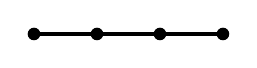
\begin{tikzpicture}[scale=0.8]
    \draw[very thick] (0,0)--(3,0);
    \foreach \x in {0,...,3} { \fill (\x,0) circle (0.1cm); }
  \end{tikzpicture}\hspace{0.5cm}
  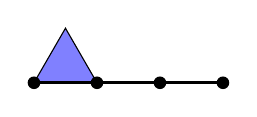
\begin{tikzpicture}[scale=0.8]
    \foreach \x/\y in {0/0} {
      \draw[fill=blue!50] (\x + \y/2, {\y*sqrt(3)/2})--(\x + \y/2 + 1/2, {(\y + 1)*sqrt(3)/2})--(\x + \y/2 + 1, {\y*sqrt(3)/2})--cycle;
    }
    \draw[very thick] (0,0)--(3,0);
    \foreach \x in {0,...,3} { \fill (\x,0) circle (0.1cm); }
  \end{tikzpicture}\hspace{0.5cm}
  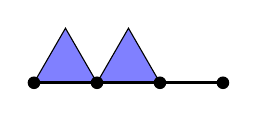
\begin{tikzpicture}[scale=0.8]
    \foreach \x/\y in {0/0, 1/0} {
      \draw[fill=blue!50] (\x + \y/2, {\y*sqrt(3)/2})--(\x + \y/2 + 1/2, {(\y + 1)*sqrt(3)/2})--(\x + \y/2 + 1, {\y*sqrt(3)/2})--cycle;
    }
    \draw[very thick] (0,0)--(3,0);
    \foreach \x in {0,...,3} { \fill (\x,0) circle (0.1cm); }
  \end{tikzpicture}\hspace{0.5cm}
  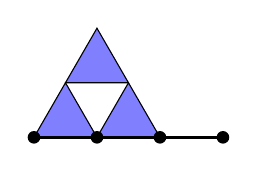
\begin{tikzpicture}[scale=0.8]
    \foreach \x/\y in {0/0, 1/0, 0/1} {
      \draw[fill=blue!50] (\x + \y/2, {\y*sqrt(3)/2})--(\x + \y/2 + 1/2, {(\y + 1)*sqrt(3)/2})--(\x + \y/2 + 1, {\y*sqrt(3)/2})--cycle;
    }
    \draw[very thick] (0,0)--(3,0);
    \foreach \x in {0,...,3} { \fill (\x,0) circle (0.1cm); }
  \end{tikzpicture}\hspace{0.5cm}
  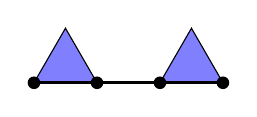
\begin{tikzpicture}[scale=0.8]
    \foreach \x/\y in {0/0, 2/0} {
      \draw[fill=blue!50] (\x + \y/2, {\y*sqrt(3)/2})--(\x + \y/2 + 1/2, {(\y + 1)*sqrt(3)/2})--(\x + \y/2 + 1, {\y*sqrt(3)/2})--cycle;
    }
    \draw[very thick] (0,0)--(3,0);
    \foreach \x in {0,...,3} { \fill (\x,0) circle (0.1cm); }
  \end{tikzpicture}\hspace{0.5cm}
  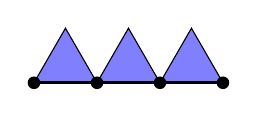
\begin{tikzpicture}[scale=0.8]
    \foreach \x/\y in {0/0, 1/0, 2/0} {
      \draw[fill=blue!50] (\x + \y/2, {\y*sqrt(3)/2})--(\x + \y/2 + 1/2, {(\y + 1)*sqrt(3)/2})--(\x + \y/2 + 1, {\y*sqrt(3)/2})--cycle;
    }
    \draw[very thick] (0,0)--(3,0);
    \foreach \x in {0,...,3} { \fill (\x,0) circle (0.1cm); }
  \end{tikzpicture}\hspace{0.5cm}
  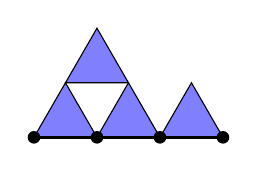
\begin{tikzpicture}[scale=0.8]
    \foreach \x/\y in {0/0, 1/0, 2/0, 0/1} {
      \draw[fill=blue!50] (\x + \y/2, {\y*sqrt(3)/2})--(\x + \y/2 + 1/2, {(\y + 1)*sqrt(3)/2})--(\x + \y/2 + 1, {\y*sqrt(3)/2})--cycle;
    }
    \draw[very thick] (0,0)--(3,0);
    \foreach \x in {0,...,3} { \fill (\x,0) circle (0.1cm); }
  \end{tikzpicture}\hspace{0.5cm}
  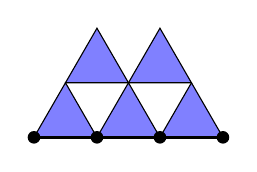
\begin{tikzpicture}[scale=0.8]
    \foreach \x/\y in {0/0, 1/0, 2/0, 0/1, 1/1} {
      \draw[fill=blue!50] (\x + \y/2, {\y*sqrt(3)/2})--(\x + \y/2 + 1/2, {(\y + 1)*sqrt(3)/2})--(\x + \y/2 + 1, {\y*sqrt(3)/2})--cycle;
    }
    \draw[very thick] (0,0)--(3,0);
    \foreach \x in {0,...,3} { \fill (\x,0) circle (0.1cm); }
  \end{tikzpicture}\hspace{0.5cm}
  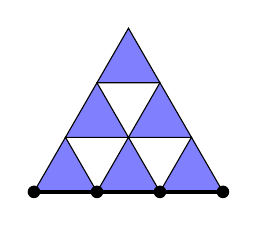
\begin{tikzpicture}[scale=0.8]
    \foreach \x/\y in {0/0, 1/0, 2/0, 0/1, 1/1, 0/2} {
      \draw[fill=blue!50] (\x + \y/2, {\y*sqrt(3)/2})--(\x + \y/2 + 1/2, {(\y + 1)*sqrt(3)/2})--(\x + \y/2 + 1, {\y*sqrt(3)/2})--cycle;
    }
    \draw[very thick] (0,0)--(3,0);
    \foreach \x in {0,...,3} { \fill (\x,0) circle (0.1cm); }
  \end{tikzpicture}
  \caption{
    All towers of equilateral triangles on a platform of width $3$.
  }
\end{figure}

\begin{figure}[!h]
  \centering
  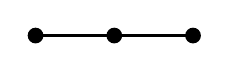
\begin{tikzpicture}
    \draw[very thick] (0,0)--(2,0);
    \foreach \x in {0,...,2} { \fill (\x,0) circle (0.1cm); }
  \end{tikzpicture}\hspace{0.5cm}
  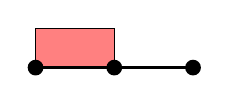
\begin{tikzpicture}
    \foreach \x/\y in {0/0} {
      \draw[fill=red!50] (\x + \y/2, \y/2) rectangle (\x + 1 + \y/2, {(\y + 1)/2});
    }
    \draw[very thick] (0,0)--(2,0);
    \foreach \x in {0,...,2} { \fill (\x,0) circle (0.1cm); }
  \end{tikzpicture}\hspace{0.5cm}
  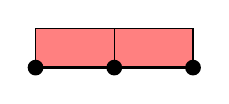
\begin{tikzpicture}
    \foreach \x/\y in {0/0,1/0} {
      \draw[fill=red!50] (\x + \y/2, \y/2) rectangle (\x + 1 + \y/2, {(\y + 1)/2});
    }
    \draw[very thick] (0,0)--(2,0);
    \foreach \x in {0,...,2} { \fill (\x,0) circle (0.1cm); }
  \end{tikzpicture}\vspace{0.5cm}\\
  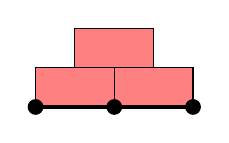
\begin{tikzpicture}
    \foreach \x/\y in {0/0,1/0,0/1} {
      \draw[fill=red!50] (\x + \y/2, \y/2) rectangle (\x + 1 + \y/2, {(\y + 1)/2});
    }
    \draw[very thick] (0,0)--(2,0);
    \foreach \x in {0,...,2} { \fill (\x,0) circle (0.1cm); }
  \end{tikzpicture}\hspace{0.5cm}
  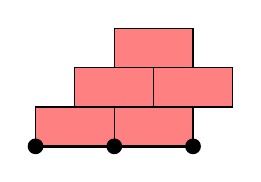
\begin{tikzpicture}
    \foreach \x/\y in {0/0,1/0,0/1,1/1,0/2} {
      \draw[fill=red!50] (\x + \y/2, \y/2) rectangle (\x + 1 + \y/2, {(\y + 1)/2});
    }
    \draw[very thick] (0,0)--(2,0);
    \foreach \x in {0,...,2} { \fill (\x,0) circle (0.1cm); }
  \end{tikzpicture}
  \caption{
    All five towers of length $2$ bricks on a length $4$ platform.
    (No row can be a vertical shift of another row, otherwise arbitrarily tall
    stacks are possible.)
  }
\end{figure}

\begin{question}
  How many different stacks exist for these shapes?
\end{question}
\begin{related}
  \item What if 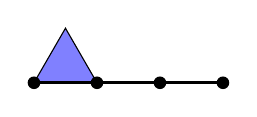
\begin{tikzpicture}[scale=0.8]
    \foreach \x/\y in {0/0} {
      \draw[fill=blue!50] (\x + \y/2, {\y*sqrt(3)/2})--(\x + \y/2 + 1/2, {(\y + 1)*sqrt(3)/2})--(\x + \y/2 + 1, {\y*sqrt(3)/2})--cycle;
    }
    \draw[very thick] (0,0)--(3,0);
    \foreach \x in {0,...,3} { \fill (\x,0) circle (0.1cm); }
  \end{tikzpicture} and 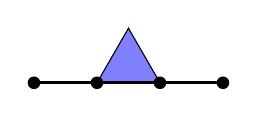
\begin{tikzpicture}[scale=0.8]
    \foreach \x/\y in {1/0} {
      \draw[fill=blue!50] (\x + \y/2, {\y*sqrt(3)/2})--(\x + \y/2 + 1/2, {(\y + 1)*sqrt(3)/2})--(\x + \y/2 + 1, {\y*sqrt(3)/2})--cycle;
    }
    \draw[very thick] (0,0)--(3,0);
    \foreach \x in {0,...,3} { \fill (\x,0) circle (0.1cm); }
  \end{tikzpicture} are considered to be distinct?
  \item What if 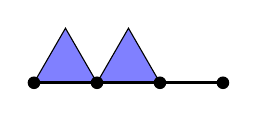
\begin{tikzpicture}[scale=0.8]
    \foreach \x/\y in {0/0,1/0} {
      \draw[fill=blue!50] (\x + \y/2, {\y*sqrt(3)/2})--(\x + \y/2 + 1/2, {(\y + 1)*sqrt(3)/2})--(\x + \y/2 + 1, {\y*sqrt(3)/2})--cycle;
    }
    \draw[very thick] (0,0)--(3,0);
    \foreach \x in {0,...,3} { \fill (\x,0) circle (0.1cm); }
  \end{tikzpicture} and 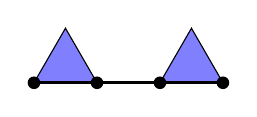
\begin{tikzpicture}[scale=0.8]
    \foreach \x/\y in {0/0,2/0} {
      \draw[fill=blue!50] (\x + \y/2, {\y*sqrt(3)/2})--(\x + \y/2 + 1/2, {(\y + 1)*sqrt(3)/2})--(\x + \y/2 + 1, {\y*sqrt(3)/2})--cycle;
    }
    \draw[very thick] (0,0)--(3,0);
    \foreach \x in {0,...,3} { \fill (\x,0) circle (0.1cm); }
  \end{tikzpicture} are considered to be the same (because one turns into the
    other by ``sliding''.)
  \item What if ``upside-down'' triangles can be placed in the gaps?
  \item What if ``upside-down'' triangles \textit{must} be placed in the gaps in
    order to stack on top?
  \item What about bricks of length 3?
  \item What about tetrahedrons and cuboids?
  \item What if the number of bricks is the constraint instead of the size of
    the platform?
\end{related}
\begin{note}
  The triangle stacking problem appears to be counted by Catalan numbers.
  If cantilevers are not allowed, the brick stacking problem reduces to the
  triangle stacking problem.
\end{note}

\end{document}
